\documentclass[12pt]{ctexart}
\usepackage[doublespacing]{setspace}
\usepackage{amsmath, amssymb}
\usepackage{graphicx}

\begin{titlepage}
    \title{智能手机销量随价格变化关系探究}
\end{titlepage}

\begin{document}

\title{智能手机销量随价格变化关系探究}                                  

\section{摘要}

    智能手机市场经过了几十年来的进化,从直板机、翻盖机到如今的全面屏手机、折叠屏手机。随着普及度越来越高,价格范围也越来越广。虽说消费者在购买手机时会受到多种因素的影响,但若是将考虑范围限定在同一品牌的手机中,便可以忽视品牌、消费人群等因素,单纯考虑\textbf{销量与手机价位的关系}。

    本文选取了\textbf{近三年来苹果手机iPhone在京东平台的销售数据},以某台售出手机的价格为随机变量,构造随机变量序列。在中心极限定理的保证下,该随机变量序列应服从正态分布;通过估计正态分布参数,得出均值和方差;通过理论计算所得的均值和方差,对苹果产品定价的合理性进行评估,并分析其它因素存在的影响。


\section{正文}

    \subsection{数据获取与初步筛选}

        \subsubsection{青睐价位数据}   

            根据京东手机页面销售数据:将手机价格划分为廉价(1-349)、低(349-1362)、中(1362-3573)、高(3573-8096)、昂贵(大于8096)(单位/元),对应手机消费者青睐比例如下表所示:

            \begin{center}
                \begin{tabular}{|c|ccccc|}
                    \hline
                    价格划分&廉价&低&中&高&昂贵\\
                    \hline
                    青睐比例&0.08&0.29&0.43&0.15&0.05\\
                    \hline
                \end{tabular}
            \end{center}

        \subsubsection{各季度iPhone销量}

            根据macstories网站整理,iPhone四季度销量呈周期性变化,且规律较为统一。

            \begin{center}
                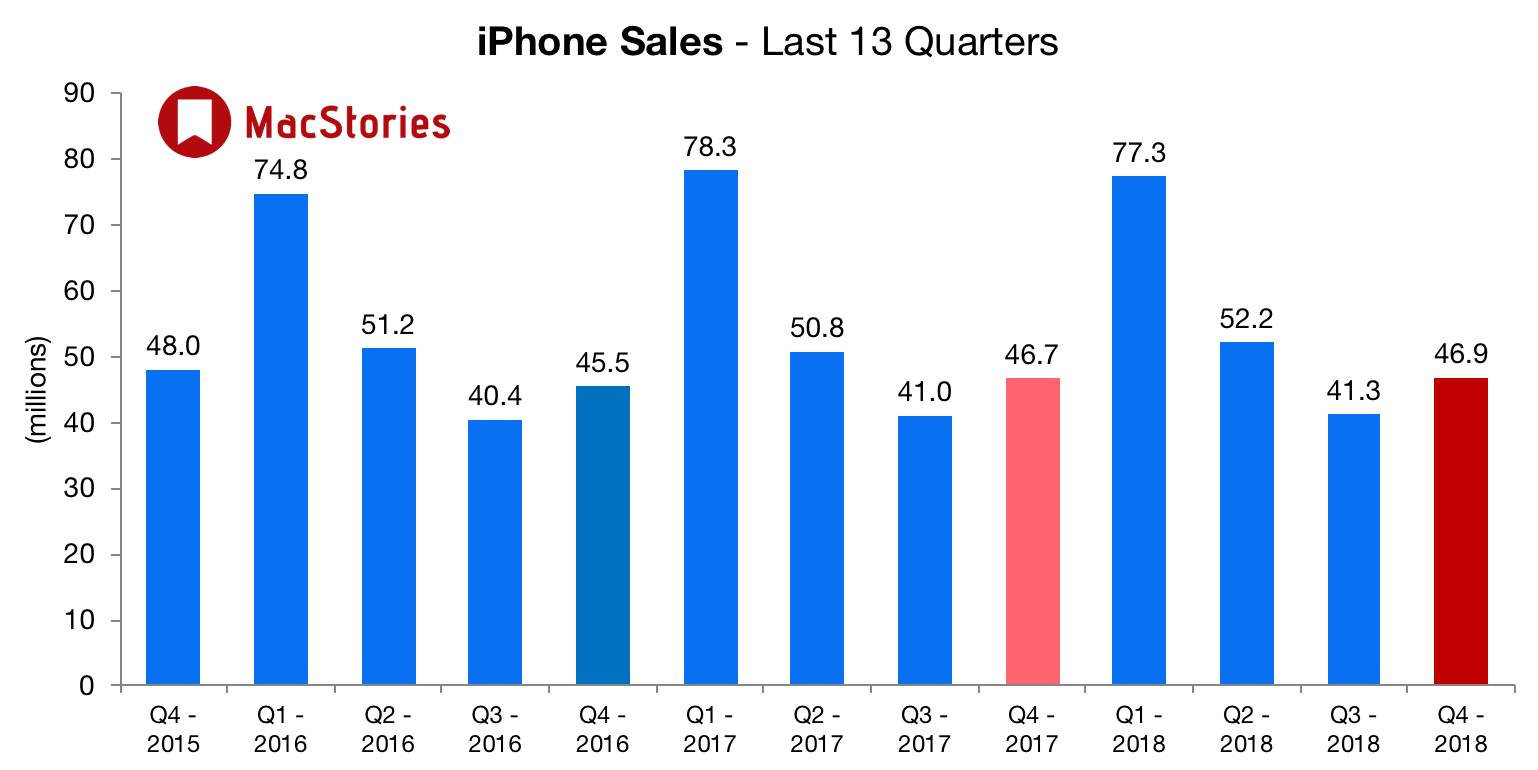
\includegraphics[width=13cm]{quarters.jpg}
            \end{center}

            因此可以对不同批次发布的产品的销量加权后进行比较,权值通过取三年每季度总销量和三年总销量之比获得。

            \begin{equation} %推荐使用equation表达式  
                \alpha _i= \frac{\sum\limits_{k = 2016}^{2018} E _{ki} }{ \sum\limits_{k = 2016}^{2018} \sum\limits_{j = 1}^{4}E _{kj} }, \qquad i=1,2,3,4
            \end{equation} 

            其中$\alpha _i$表示第$i$个季度的权值,$E _{ki}$ 为第$k$年第$i$季度的销量。

            \begin{center}
                \begin{tabular}{|c|c|c|c|c|}
                    \hline
                    季度 $i$ & 一&二&三&四\\
                    \hline
                    权重 $\alpha _i$&0.356 &0.239&0.190 &0.215\\
                    \hline
                \end{tabular}
            \end{center}

            \begin{center}
                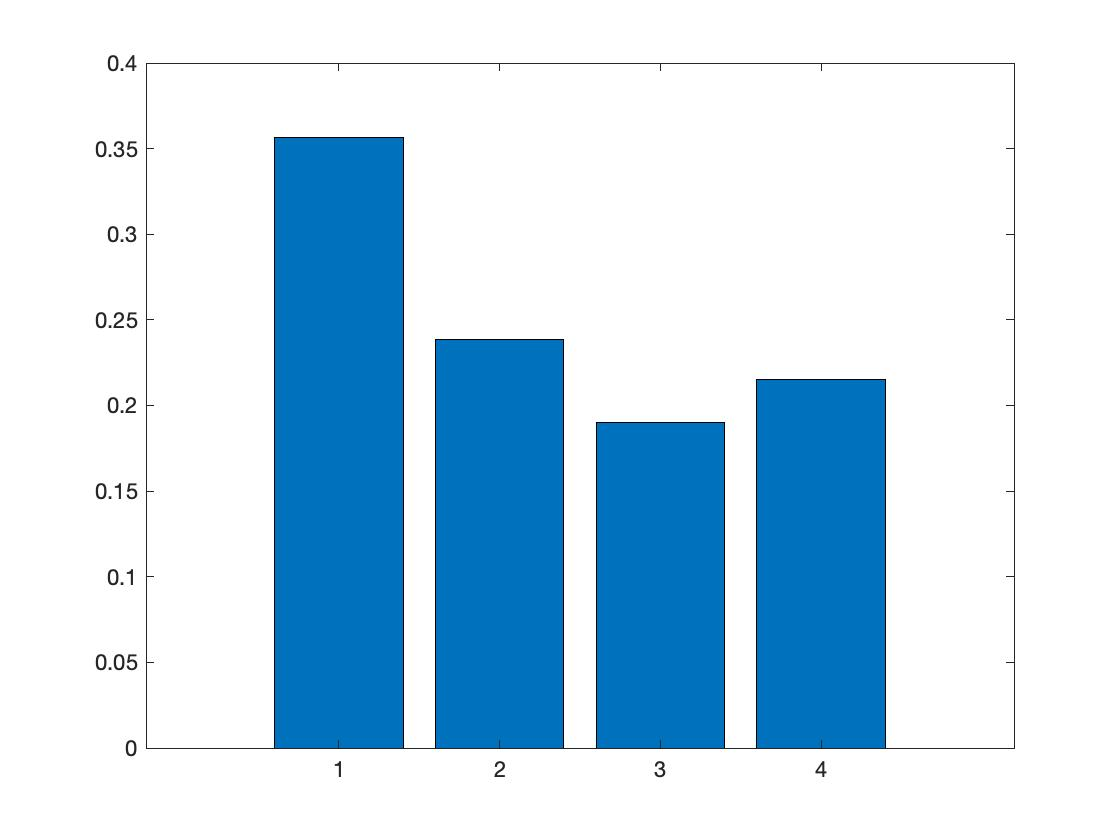
\includegraphics[width=9cm]{per-quaters.jpg}
            \end{center}
             

        \subsection{各产品总销量}

            每款iPhone销量通过京东的评价数得出;
            其价格通过软件「慢慢买」得出售价的波动曲线。
            因新手机在上市第一季度售价相对稳定,通过四季度销量分布可以折算出每款手机在发布后第一个季度的销量(即第四季度),使不同时间发布的手机具有一定的可比性。

            \begin{equation} %推荐使用equation表达式  
                E _i ' = \alpha _4 \cdot  E _i
            \end{equation} 

            

            \begin{center}
                \begin{tabular}{|c|ccc|}
                    \hline
                    2019.9上市机型 & 上市价格/元 & 总销量/万台 & 折算销量/万台\\
                    \hline
                    iPhone 11 &5999 &70 &70\\
                    \hline
                    iPhone 11 Pro&9999 &13&13\\
                    \hline
                    iPhone 11 ProMax&10899 &12&12\\
                    \hline
                \end{tabular}

                \begin{tabular}{|c|ccc|}
                    \hline
                    2018.9上市机型 & 上市价格/元 & 总销量/万台 & 折算销量/万台\\
                    \hline
                    iPhone XR  &6999 &208 &44\\
                    \hline
                    iPhone Xs &8699 &36&7\\
                    \hline
                    iPhone Xs Max&10999 &103&22\\
                    \hline
                \end{tabular}
                
                \begin{tabular}{|c|ccc|}
                    \hline
                    2017.9上市机型 & 上市价格/元 & 总销量/万台 & 折算销量/万台\\
                    \hline
                    iPhone 8 &4777 &152 &21\\
                    \hline
                    iPhone 8 Plus &6899 &199&32\\
                    \hline
                \end{tabular}
            \end{center}

\subsection{数据处理与参数估计}
    
    
    
    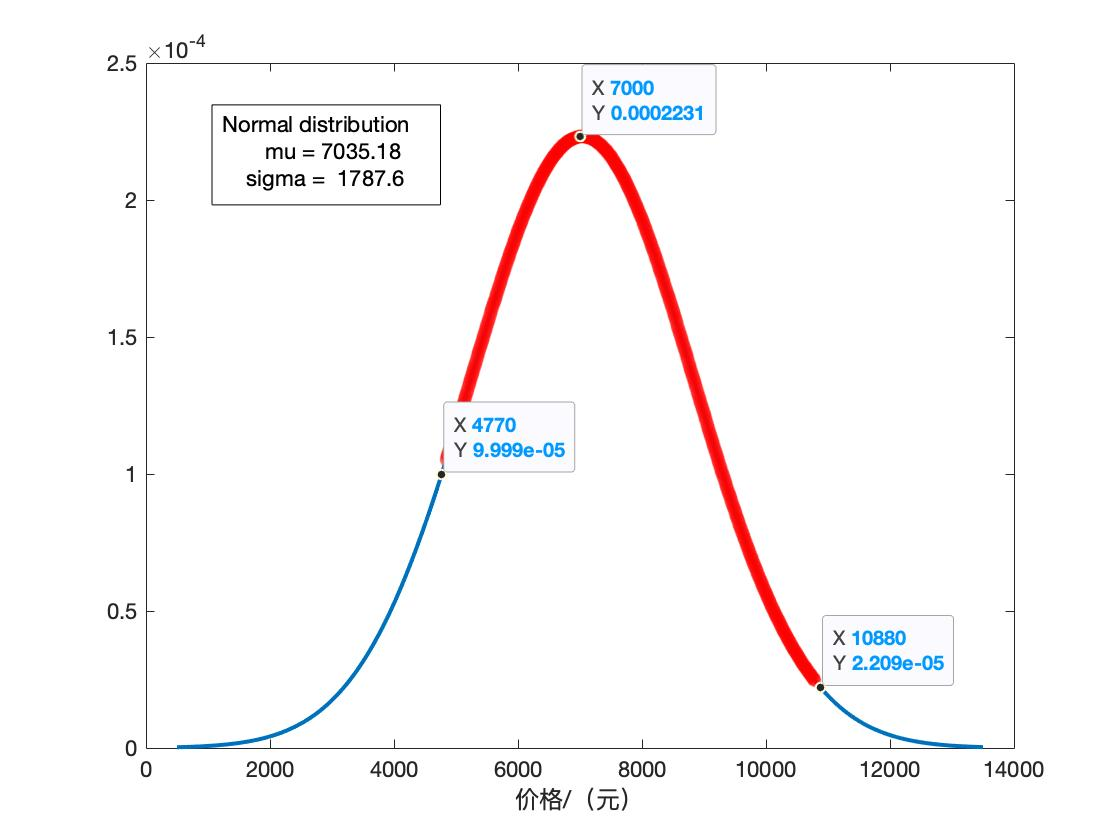
\includegraphics[width=12cm]{price_normal_distribution.jpg}



\section{分析与结论}


\end{document}

